\section{Verallgemeinerte Darstellung des Regelungsproblem}
Im ersten Schritt wird eine allgemeine Modellform eingeführt, für welche ein Teil der Entwurfsprobleme optimal gelöst werden kann. In späteren Anwedungsfällen wird die Problemstellung in die allgemeine Form überführt und anschließend gelöst. Die Darstellung setzt sich aus einem erweiterten Streckenmodell $P$ und einem Regler $K$ zusammen. In die Strecke $P$ gehen sowohl der letztendliche Stellvektor $\vec{u}$ als auch der exogene Vektor $\vec{w}$ ein. Die Strecke gibt wiederum den exogenen Vektor $\vec{z}$ als auch den gemessenen Führungsvektor $\vec{y}$ aus, welcher in den Regler $K$ geführt wird um wiederum den Stellvektor $\vec{u}$ zu berechnen.

\begin{figure}[h!]
\centering
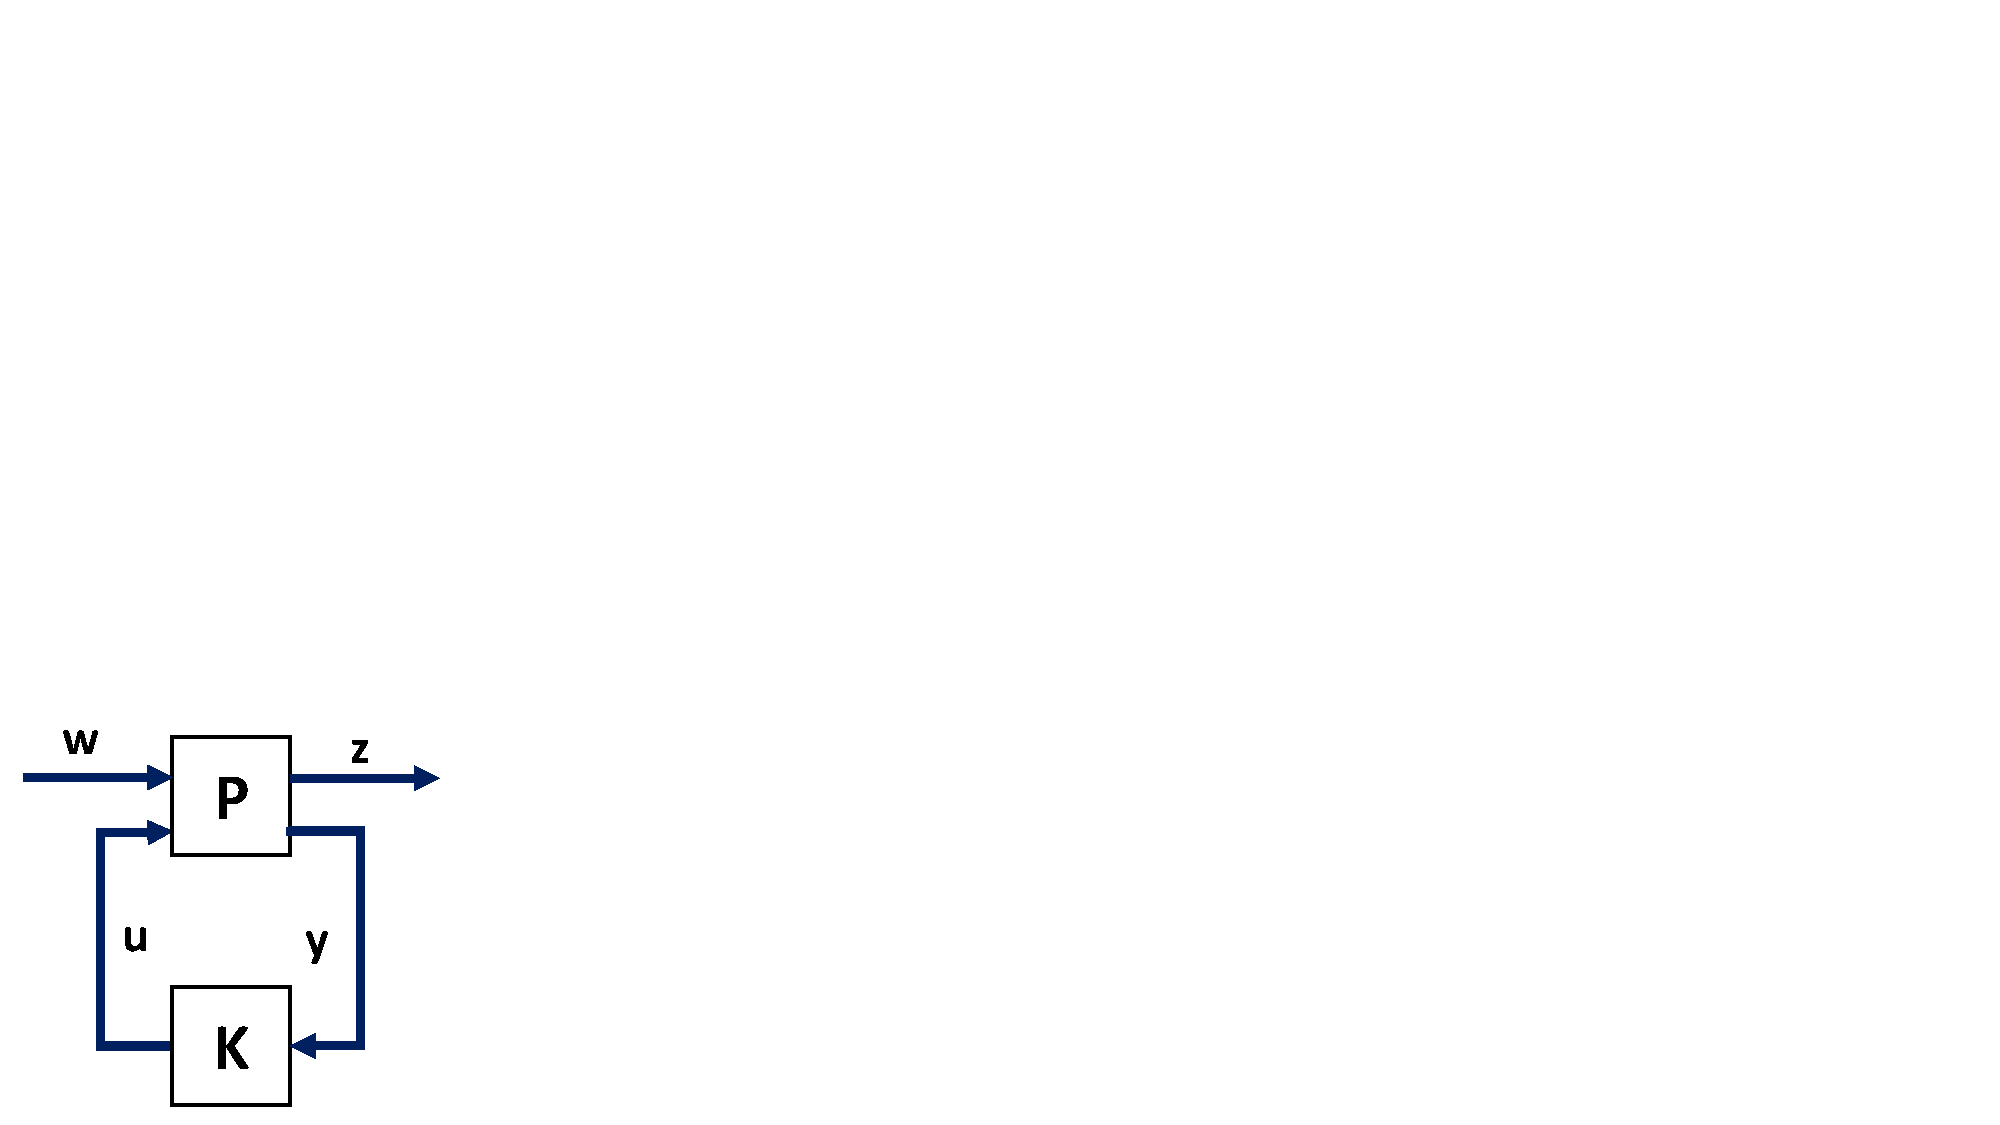
\includegraphics[trim={0 0 25cm 12cm}, clip, width=0.3\linewidth]{img/StandardControlProblem_BSB}
\caption{Verallgemeinerte Darstellung des Regelungsproblems}
\end{figure}

Aus dem Blockschaltbild ergibt sich 
\begin{equation}
\begin{bmatrix}
\vec{z} \\ \vec{y}
\end{bmatrix} = P(s)\cdot \begin{bmatrix}
\vec{w} \\ \vec{u}\end{bmatrix} = \begin{bmatrix}
P_{11}(s) & P_{12}(s) \\ P_{21}(s) & P_{22}(s)
\end{bmatrix}\cdot \begin{bmatrix}
\vec{w} \\ \vec{u}
\end{bmatrix}
\end{equation}
\begin{equation}
\vec{u} = K(s)\cdot \vec{y}
\end{equation}
für den Zusammenhang zwischen verallgemeinerter Strecke und Regler. Die Übertragungsfunktion von $\vec{w}$ zu $\vec{z}$ im geschlossenen Regelkreis folgt mit
\begin{equation}
\vec{z} = F_l(P,K)\cdot \vec{w}; \hspace{35pt} F_l(P,K) = P_{11} + P_{12}K(I - P_{22}K)^{-1}P_{21}\,.
\end{equation}